\chapter{Problématique et contraintes}



\section{Généralités}
Afin de fonctionner correctement et d'être efficace pour une population donnée, un algorithme de recommandation fait face à un certain nombre de contraintes selon son type : 


\vspace{5mm}


\begin{itemize}
    \item \textbf{Item cold start} : C'est lorsqu'un item est nouveau ou simplement lorsque l’item n’a pas encore été « cliqué » ou « acheté ». Cet item est difficilement recommandable via des algorithmes de recommandation de type collaborative filtering. En employant des méthodes de type content-based un nouvel item est facilement recommandable même si cet item est nouveau.
    \vspace{2mm}
    \item \textbf{User cold start} : Si un utilisateur est nouveau, il existe aucun historique d’interaction avec le système. Il faut alors avoir recours à des données extérieures pour pouvoir commencer à recommander des items pertinents comme des données extraites des réseaux sociaux ou une demande explicite des goûts des nouveaux utilisateurs.  
    \vspace{2mm}
    \item \textbf{Diversity} : Ce problème survient souvent lors de l’utilisation de méthodes de type "contentbased filtering", le système recommande toujours les mêmes items à un utilisateur, ce qui l’enferme sans possibilité d’exploration en dehors des intérêts détectés par le système.
    \vspace{2mm}
    \item \textbf{Grey sheep} : certains utilisateurs ne font rien comme les autres, on ne peut donc pas leur recommander d’item via les méthodes de type collaborative filtering. 
    \vspace{2mm}
    \item \textbf{Quality} : le content based filtering analyse le contenu, mais la qualité du produit n'est pas forcement déterminé par son contenu (A survey on recommendation system de Singh et al.).
    \vspace{2mm}
    \item \textbf{Trust} : les utilisateurs doivent avoir confiance et croire en la performance du système pour continuer à l’utiliser.
    
\end{itemize}

\vspace{5mm}

Il existe un grand nombre d’autres contraintes comme \textbf{Scalability}, \textbf{Privacy}, et bien d’autres.



\section{Les contraintes et problématiques de Netflix}


A la création d'un compte Netflix, pour contourner le problème de l’\textbf{User Cold Start} le système demande à l'utilisateur de choisir un ensemble de séries ou de films qu'il aime déjà. Ainsi le système de recommandation de Netflix peut commencer à recommander d'autres contenus. Les contenus recommandés doivent être de bonne qualité (contrainte \textbf{Quality}) sinon l’utilisateur lassé n’utilisera plus le service. 

\vspace{5mm}

Chaque mois, Netflix met à disposition de nouveaux programmes originaux sur sa plateforme et donc se retrouve face à la contrainte \textbf{Item-Cold-Start}. Ce contenu étant nouveau, il manque d’avis permettant de déterminer sa qualité. Les programmes sont ainsi mis en avant par la plateforme pour faire leurs promotions mais aussi dans les strates de recommandation en fonction des mots-clés associés. 

\vspace{5mm}

Les abonnements étant mensuels et sans engagement, chaque mois Netflix doit convaincre les utilisateurs de rester sur la plateforme. Ainsi de façon mensuelle, la plateforme subie les contraintes \textbf{Diversity} et \textbf{Trust}. En offrant de nouveaux contenus chaque mois, la plateforme doit convaincre ses utilisateurs que la recommandation est pertinante vis à vis de leurs besoins.

 



\section{L'importance de la recommandation pour Netflix}

%https://medium.com/netflix-techblog/artwork-personalization-c589f074ad76

Avec un catalogue composé de milliers de films et de séries par pays ainsi qu’une base d’utilisateurs grandissante de plusieurs millions d’utilisateurs à travers le monde, il est difficile pour Netflix d’utiliser un unique algorithme pour recommander des contenus.

\vspace{5mm}

Dans un article publié par Netflix\supercite{netflixRS&BusinessValue}, les auteurs (responsables du machine learning chez Netflix) font l'état de six algorithmes présents sur la page d’accueil afin d’afficher une recommandation unique à chaque utilisteur : 

\vspace{5mm}


\begin{itemize}
    \item \textit{« Le \textbf{"Personalized Video Ranker"} opère le classement personnalisé des vidéos et ordonne les 40 rangées de 75 titres qui composent la page d’accueil.}
    
    \vspace{2mm}
    
    \item \textit{Le \textbf{"Top-N Video Ranker"} sélectionne, parmi les contenus les plus populaires dans l’ensemble du catalogue, ceux susceptibles de plaire à l’utilisateur.}
    
    \vspace{2mm}
    
    \item \textit{Le \textbf{"Trending Now"} détermine les tendances à court terme chez les consommateurs : les comédies romantiques de la Saint-Valentin ou les films de Noël, par exemple.}
    
    \vspace{2mm}
    
    \item \textit{Le \textbf{"Continue Watching"} sélectionne les vidéos que l’utilisateur a commencé à regarder et dont il souhaite probablement reprendre la lecture.}
    
    \vspace{2mm}
    
    \item \textit{Le \textbf{"Video-Video Similarity"} choisit les vidéos susceptibles de plaire à un utilisateur, compte tenu des similitudes existantes entre elles et celles qu’il a regardées.}
    
    \vspace{2mm}
    
    \item \textit{Le \textbf{"Page Generation : Row Selection and Ranking"} détermine les rangées à faire figurer sur la page d’accueil et leur ordre d’apparition, en tenant compte des résultats des algorithmes précédents.»}\supercite{franceInfoEnq}
   
\end{itemize}

\vspace{5mm}

%http://www.internetactu.net/2017/10/25/tout-est-recommandation-comment-netflix-sest-transforme/

Selon leurs études, un utilisateur de Netflix doit mettre au maximum 90 secondes à choisir un film, au-delà il perd de l'intérêt pour la plateforme. Pour Netflix, cela correspond entre 10 et 20 films proposés ou recommandés. Dans ce cas, si un utilisateur ne lance pas de film, il quitte le service. Le risque à terme est que l’expérience se renouvelle pour un utilisateur et qu’il ne soit plus satisfait de la proposition du contenu et se désabonne. 

\vspace{5mm}

\begin{figure}[htp]
  \centering
  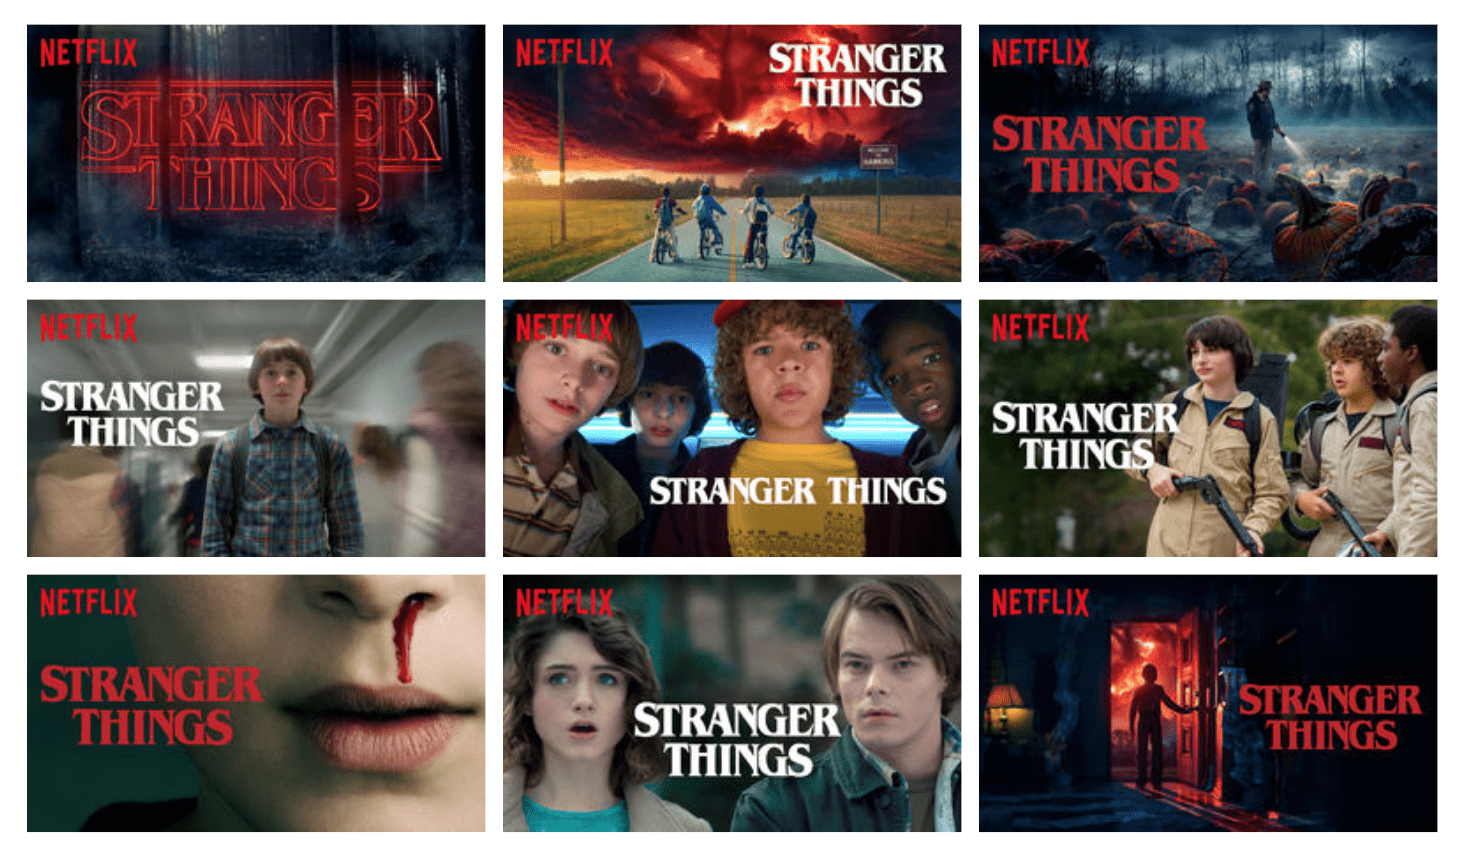
\includegraphics[width=80mm]{./src_img/strangerthings}
  \caption{Exemple de la diversité des illustrations.\supercite{franceInfoEnq}}
  \label{fig:deux-trois}
\end{figure}

\vspace{5mm}

Personnaliser la page d’accueil afin de la rendre unique pour chaque utilisateur est une première étape dans la stratégie de recommandation de Netflix. Lorsqu’un utilisateur navigue dans l’interface, il faut le convaincre de consommer un contenu en moins de 90 secondes.  
Pour rendre sa recommandation plus attractive et personnelle à chaque utilisateur, Netflix a commencé à produire plusieurs illustrations pour chaque contenu. Chaque illustration doit faire ressentir une émotion différente permettant de faire correspondre la vignette du contenu mis en avant avec les goûts de l’abonné.


\vspace{5mm}

\begin{figure}[htp]
  \centering
  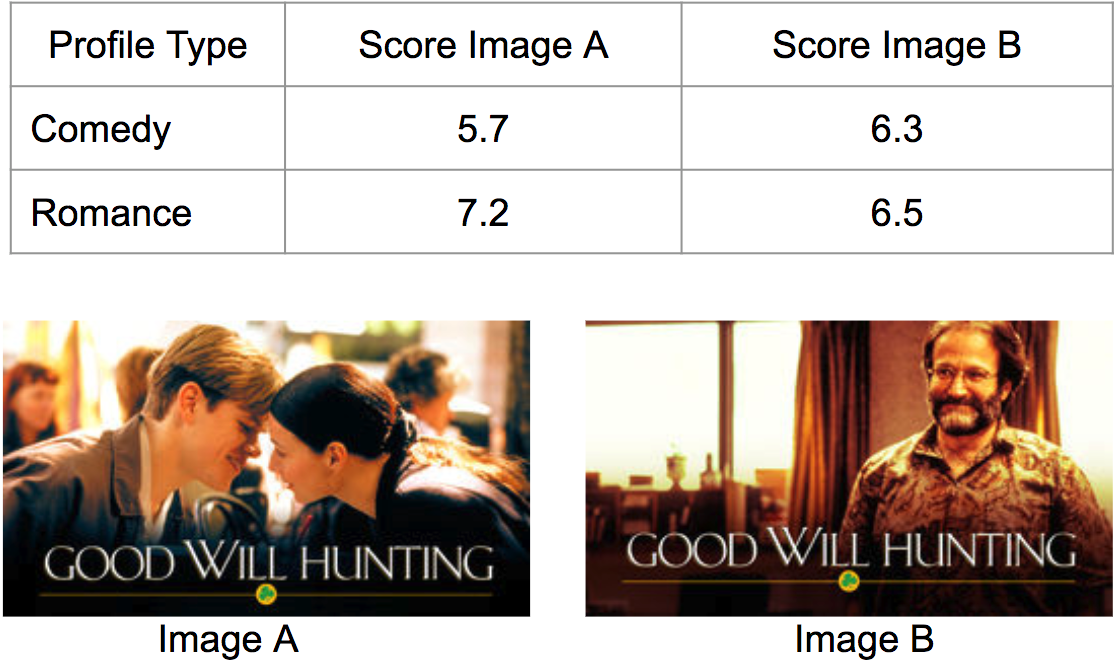
\includegraphics[width=95mm]{./src_img/score}
  \caption{Exemple de score et profil pour le film "Good Will Hunting" .}
  \label{fig:deux-quatre}
\end{figure}

\vspace{5mm}

Si nous prenons l’exemple du film, Good Will Hunting qui est une comédie romantique. 
Un profil qui est déterminé comme regardant principalement des comédies, l’algorithme va choisir la vignette du film mettant en avant Robin Williams un acteur célèbre pour des comédies comme Madame Doubfire par exemple. A l’inverse, si un abonné est déterminé comme préfèrant les contenus romantiques, c’est alors l'image d'un couple s'embrassant qui est choisie. Pour chaque vignette, un ensemble de méthode détermine la correspondance sur 10 de chaque illustration avec chaque type (comédie, romance, horreur, science fiction,...). L'algorithme choisit pour chaque profil d'utilisateur, l'illustration qui correspond le mieux à ses goûts. Cette étape est déterminée par le type qui correspond à l'utilisateur et le score de l'illustration le plus élevé pour ce type de profil.  

\vspace{5mm}

En plus de cibler ses abonnés et grâce à ses multiples vignettes pour une seule série, Netflix peut tester la vignette la plus efficace. Permettant ainsi de proposer les vignettes les plus efficaces pour un nouvel abonné mais aussi d’agrandir la fanbase d’une série. Un fan sur cinq\supercite{1/5} de Stranger Things n’avait jamais regardé de contenus horrifiques sur Netflix. 

\vspace{5mm}

Début 2019, Netflix à dévoilé ses résultats trimestriels. Dans ce communiqué\supercite{fornite}, Netflix affirme que ses principaux rivaux sont désormais Fortnite et YouTube. L’entreprise explique que sa présence globale sur les écrans est supérieure à HBO (chaîne qui possède Game of Thrones) mais inférieure à celle de Fornite le phénomène incontesté du jeux vidéo en 2018. Le temps utilisé pour jouer à Fornite n’est pas utilisé pour regarder des séries, des films ou des documentaires sur Netflix. On parle ici d’une bataille de l’attention et finalement d’argent. En effet : l’argent dépensé pour acheter des tenues dans Fornite n’est pas de l’argent investi dans un abonnement mensuel pour Netflix. Ainsi, plus que jamais, Netflix doit s'appuyer sur son contenu et sur l’ensemble de son système de recommendation pour convaincre ses utilisateurs de consommer sur leur site et donc de passer du temps sur leur plateforme plutôt que de jouer à Fornite pour gagner la bataille de l'attention. 


%https://medium.com/netflix-techblog/artwork-personalization-c589f074ad76


%https://www.sciencesetavenir.fr/high-tech/data/comment-l-algorithme-de-netflix-vous-rend-accro_115965

%https://usbeketrica.com/article/netflix-personnalisation-illustrations-algorithme
